\documentclass[12pt]{article}


% ========================================================================
% preamble
% ========================================================================

% (stuff that you don't have to mess with or worry about right now.)
%\setlength{\topmargin}{-.25in}
%\setlength{\headheight}{0in}
%\setlength{\headsep}{0in}
%\setlength{\oddsidemargin}{-.3in}
%\setlength{\textwidth}{7truein}
%\setlength{\textheight}{10.0truein}

% packages for fancy fonts, symbols, thm/proof environments, etc
\usepackage{amsmath,amssymb,amsthm}
\usepackage{graphicx}
\usepackage{mathrsfs}
\usepackage[margin=1in]{geometry}
\usepackage{hyperref}

\usepackage{parskip}

%For the lazy:
\newcommand{\ds}{\displaystyle}
\newcommand{\tbf}{\textbf}
\newcommand{\ti}{\textit}
\newcommand{\mC}{\mathcal}
\newcommand{\mB}{\mathbb}

\newcommand{\mrm}{\mathrm}
\newcommand{\dds}[2]{\frac{\mathrm{d}#2}{\mathrm{d}#1}} %(d1 BY d2)
\newcommand{\ddb}[2]{\frac{\mathrm{d}}{\mathrm{d}#1}\left[ #2\right]}
%(d by d1 OF 2)

\begin{document}
\flushleft

\centerline{\large \bf Low Rank Factorization Using Error Correcting Codes}
\centerline{\large \bf APPM 5720 Final Project}
\vspace{\baselineskip}
{\large \centerline{James Folberth and Jessica Gronski}}
\vspace{\baselineskip}

\section{Introduction}
In recent years, randomized techniques have gained a significant amount of attention for their simplicity and ability to efficiently generate low rank approximations of large matrices. We have discussed several randomized methods in class including the Subsampled Random Fourier and Hadamard Transforms (SRFT and SRHT, respectively). Ubaru et al. \cite{ubaru2015low} propose using error correcting codes to find low rank approximations and matrix factorizations of large matrices in a manner similar to SRFT/HT. The goal of our project is to compare their proposed method with those discussed in class for face recognition. 

\section{Error Correcting Codes}
In what follows, we give a brief overview of error correcting codes and the subspace embedding properties they satisfy. In communication systems, data are transmitted from a source (transmitter) to a destination (receiver) through physical channels. These channels are usually noisy, causing errors in the data received \cite{ubaru2015low}, and so error correcting codes were designed to help remedy this issue. BCH codes, named after  Bose, Chaudhuri, and Hocquenghem, are of specific importance for their rich structure, ability to correct multiple bit errors and ease of decoding a transmitted message. They form a class of cyclic codes; if \tbf{c} is a codeword in the linear code space $C$, then \tbf{$\tilde{c}$} is also in $C$ where \tbf{$\tilde{c}$} is a cyclic shift of \tbf{c}. 

\vspace{3mm}

A linear code $C$ can be represented by the codeword length $\ell$ and message length $r$.  For any two integers $t$ and $q$, a BCH code over the binary field $\mB{F}_2$ has length $\ell = 2^q - 1$ and dimension $r = 2^q - 1 - tq$. In order to encode a message of $r$ bits, we require $2^r$ unique code words and so $C$ has matrix dimension $2^r \times \ell$. Another feature of BCH codes is that any two codewords maintain a minimum distance of at least $2t + 1$, where we define distance as the number of positions at which the codes differ. Moreover, we can define the \ti{dual} of the code as a code of length $\ell' = 2^q - 1 = \ell$, dimension $r' = tq$ and minimum distance at least $2^{q-1} - (t -1)2^{q/2}$. The notion of a dual distance is of particular importance because a code matrix with dual distance greater than 4 will satisfy the Johnson-Lindenstrauss Transform (JLT) property and allow for an efficient subspace embedding. Therefore, for a fixed integer $q$ (fixed codeword length), the length of the message that can be transmitted through a channel efficiently depends on the value of $t$.

\section{Subsampled Code Matrix}
Let $A$ be an $m \times n$ matrix with approximate rank $k$. Similar to the randomized methods we've discussed in class, we would like to construct a lower dimensional subsampling matrix  $\Omega$ such that $Y = A \Omega $ provides a ``good" approximation for the column space of $A$. Ideally, the size of the subsampling matrix, i.e. the target rank, is much smaller than the dimension of the original matrix $A$, greatly reducing the cost of performing other factorizations like the QR or SVD on the subsampled matrix.

\vspace{3mm}
The question now is how do we construct an $\Omega$ from error correcting codes  that still preserve the geometry of the original problem? We choose the length of the message vector $r \ge \lceil{\log_2n\rceil}$ and the length of the codewords $l > k$, the target rank. Notice that $l$ will depend on the dual distance of the code. We then consider the linear coding scheme as follows: 

\[ \Omega = \sqrt{ \frac{ 2^r }{ \ell } } D S \Phi, \] 

where 
\begin{itemize}
\item $D$ is a random $n \times n$ diagonal matrix whose entries are independent random signs, i.e., random variables uniformly distributed on $\{ \pm 1 \}$.

\item $S$ is a uniformly random downsampler, an $n \times 2^r$ matrix whose $n$ rows are randomly selected from a $2^r \times 2^r$ identity matrix.

\item $\Phi$ is the $2^r \times \ell$ coding matrix, generated using an $[ \ell, r]$-linear coding scheme, with a binary phase-shift keying (BPSK) mapping and scaled by $2^{-r/2}$ such that all columns have unit norm.

\end{itemize}
Recall that the codeword matrix $C$ has $2^r$ codewords each of length $\ell$, i.e. a set of $2^r$ vectors in $\{0,1\}^{\ell}$. The BPSK mapping is defined as follows: given a codeword $\tbf{c} \in C$, $\tbf{c} \mapsto \phi \in \mB{R}$ by assigning $1 \rightarrow \frac{-1}{\sqrt{2^r}}$ and $0 \rightarrow \frac{1}{\sqrt{2^r}}$. This way, we transform the binary code matrix $C$ to the code matrix $\Phi = (\phi_1^T,  \hdots \phi_{2^r}^T) ^T$ \cite{ubaru2015low}. Moreover, it can be shown that if the dual distance is greater than or equal to 3, $\Phi$ will have orthonormal columns. The scaling factor $\sqrt{\frac{2^r}{\ell}}$ enforces the rows of $\Omega$ to also have unit length.


%TODO basically just need to type up the algorithm.  The sampling matrix is a "plugin"
\section{Prototype Algorithm}
The algorithm provided by Ubaru et al. in \cite{ubaru2015low} 


\section{RSVD Experiments}
We implemented sampling with dual BCH code matrices using various tools from the {\sc matlab} Communications System Toolbox \cite{matlab_cst_2015}.  The toolbox provides a primal BCH encoder in {\sc matlab} script.  The main operation in encoding is simulating a shift register, which is vectorized.  The toolbox also provides a function, \texttt{bchgenpoly}, which generates a vector over $\mathbb{F}_2$ that represents the generating polynomial, $F_p(x)$, for the primal BCH code.  The dual generating polynomial is 

\[ F_d(x) = \dfrac{x^l+1}{F_p(x)}, \] 

\noindent where the remainder is $0$ \cite{hall2003notes}.  Polynomial division over $\mathbb{F}_2$ is (thankfully) implemented in \texttt{deconv}, which is provided in the Communications System Toolbox.  Once we have the dual generating polynomial, we may borrow the shift register from the primal BCH encoder, and we have a functioning dual BCH encoder.

To compute the sampling matrix $\Omega$, we draw $n$ Rademacher variables to form $D$, and draw the indices of the subsampling matrix $S$.  We then compute a $n\times r$ message matrix with each row a binary vector corresponding to the decimal index from $S$.  Finally, we compute the $n\times \ell$ subsampled code matrix $S\Phi$ by encoding the message matrix with the dual BCH encoder.  To be clean, we are forming the subsampled code matrix, and use BLAS to apply it to the data matrix $A$.  We will see in the next section a method of efficiently sampling $A$ with the SRHT.

For the first experiment, we compare various sampling methods for the RSVD with oversampling parameter $p=5$ and $q=0$ power iterations.  We use the matrix \verb|LOCAL_fast_decay(100,140,200)|, which was used frequently in our homeworks.  Figure \ref{fig:rsvd_compare_fast} shows the spectral and Frobenius norms for the various sampling methods.  We can see that sampling with dual BCH code matrices are competitive with Gaussian matrices and the SRFT.  If we use $q=1$ or more power iterations, we are not able to resolve any differences between the sampling methods.

\begin{figure}[h!]
   \centering
   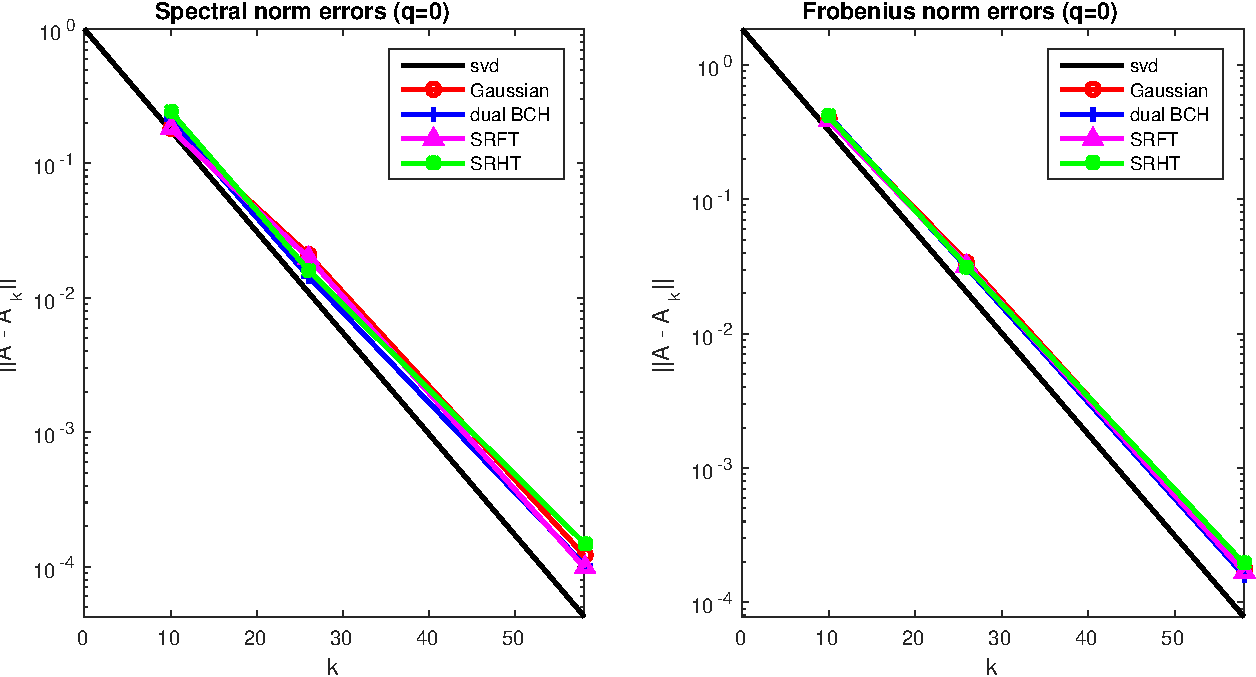
\includegraphics[width=0.9\textwidth]{figures/fast_decay_rsvd_compare_trim.pdf}
   \caption{RSVD with various sampling methods on \texttt{LOCAL\_fast\_decay(100,140,200)}.}
   \label{fig:rsvd_compare_fast}
\end{figure}

As a second experiment with the RSVD, we attempt to recreate one result from \cite{ubaru2015low}.  They selected the matrix \texttt{Kohonen.mat}, an adjacency matrix for a directed graph, from the UFL sparse matrix collection \cite{ufl_smc}.  Figure \ref{fig:rsvd_compare_kohonen} shows the spectral and Frobenius norm errors, again with oversampling $p=5$ and $q=0$ power iterations.  Notice that the singular values of \texttt{Kohonen.mat} do \emph{not} decay quickly, and so the RSVD is not accurate, regardless of sampling.  Nevertheless, dual BCH codes performed slightly better than the SRFT and Gaussian matrices.

\begin{figure}[h!]
   \centering
   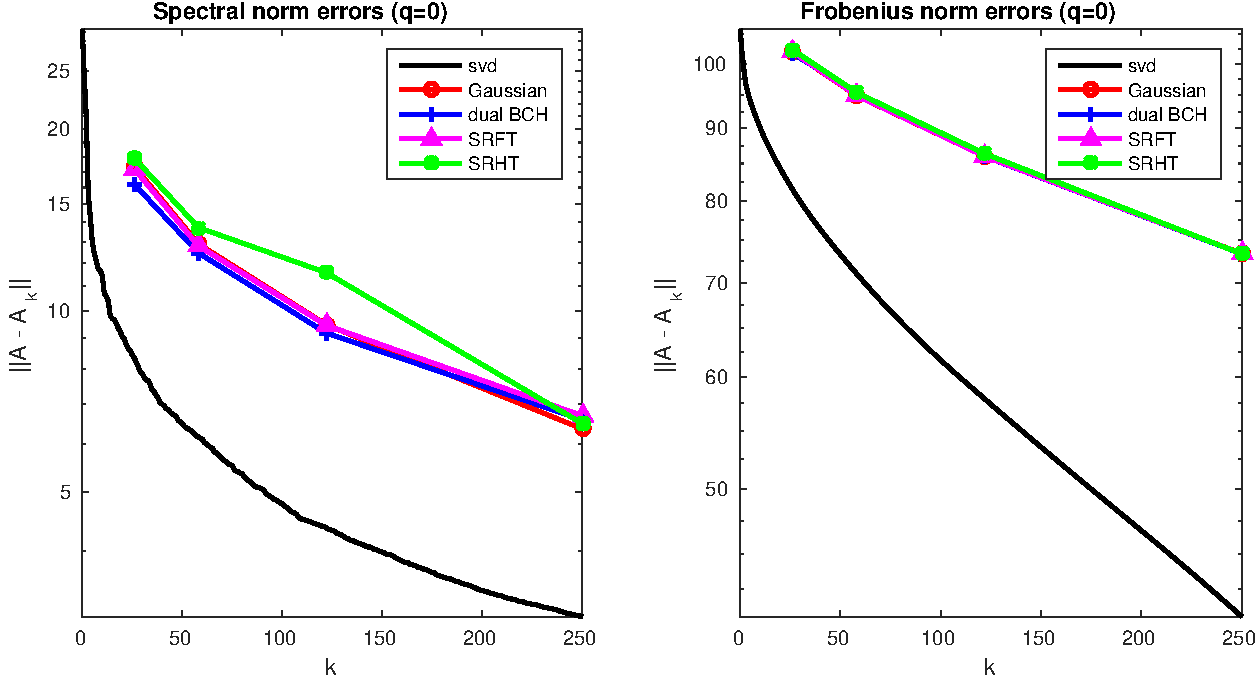
\includegraphics[width=0.9\textwidth]{figures/kohonen_rsvd_compare_trim.pdf}
   \caption{RSVD with various sampling methods on \texttt{Kohonen.mat} from \cite{ufl_smc}.}
   \label{fig:rsvd_compare_kohonen}
\end{figure}

One downside to sampling with dual BCH code matrices is the restriction of $\ell$ to $\ell=2^q-1$.  If we have a target rank of $k=100$, we must pick $p=27$ which gets us to the nearest admissible code length of $\ell=127$.  This does add a bit of work, but is offset by the existence of a fast multiplication via the SRHT, discussed in the following section.


\section{An efficient SRHT}
The naturally ordered (Walsh-)Hadamard transform is structured orthogonal transform inspired by the DFT and Haar wavelet transforms.  Neglecting normalization, it can be defined recursively for sizes $d=2^r$ as

\begin{equation}
\label{eq:had_rec}
H_1 = \begin{bmatrix}1 & 1\\1 & -1\end{bmatrix}, \quad H_d = \begin{bmatrix}H_{d/2}&H_{d/2}\\H_{d/2}&-H_{d/2}\end{bmatrix}.
\end{equation}

   \noindent Using this recursion, we also have a fast algorithm for computing the transform of a vector (or matrix, column-wise).  Notice that each Hadamard matrix $H_d$ has $\pm 1$ entries.  Recall that after the BPSK mapping, the primal and dual BCH code matrices also have $\pm 1$ entries.  In \cite{ailon2009fast} it was shown that every row of the $2^r\times \ell$ code matrix $\Phi$ is equal to some row of the $2^r\times 2^r$ Hadamard matrix, up to some normalization.  Therefore, if we do some offline preprocessing to determine the proper row subsampling for the Hadamard transform, we can use the subsampled Hadamard transform to compute sampling with subsampled dual BCH code matrices and so sampling with dual BCH codes enjoys a fast transform, just like the SRFT and SRHT.

   The recursive definition of the naturally ordered Hadamard transform (\ref{eq:had_rec}) leads naturally to an $\mathcal{O}(d\log d)$ implementation, by computing the full length $d$ transform and then subsampling to, say, $k$ indexes.  However, we can do better, although it seems that no one has implemented and made publicly available a smarter transform.
   
   Ailon and Liberty pointed out that by including the subsampling matrix in the recursion, we can reduce the complexity to $\mathcal{O}(d\log k)$, which should yield an improved runtime when $k\ll d$ \cite{ailon2009fast}.  Let $S$ be a row subsampling matrix, taking in $d$ rows and keeping only $k$ rows.  We can define the SRHT recursively as 

   \begin{equation}
      \label{eq:srht_rec}
      SH_dx = \begin{bmatrix} S_1 & S_2\end{bmatrix}\begin{bmatrix} H_{d/2} & H_{d/2}\\H_{d/2}&-H_{d/2}\end{bmatrix} \begin{bmatrix}x_1\\x_2\end{bmatrix} = S_1 H_{d/2}(x_1+x_2) + S_2H_{d/2}(x_1-x_2),
   \end{equation}

   \noindent where $x_1$ and $x_2$ are the first and second halves of $x$; $S_1$ and $S_2$ sample $k_1$ and $k_2$ rows, respectively; and $k_1+k_2=k$.  The algorithm proceeds by computing $x_1+x_2$ and $x_1-x_2$, and then recursing to compute $S_1H_{d/2}$ and $S_2H_{d/2}$.  At some point, say $d=8$, we directly compute the full $8\times 8$ transform and subsample.  We then proceed back ``up'' the recursion.  In \cite{ailon2009fast}, it was shown that this algorithm has complexity $\mathcal{O}(d\log k)$.  Recall that this means that the complexity is asymptotically bounded above by a constant times $d\log k$, not that the complexity is asymptotically a constant times $d\log k$.

We call a direct, natural implementation of either ``algorithm'' (\ref{eq:had_rec}) or (\ref{eq:srht_rec}) a reference implementation, as we will compare the runtime of any optimized implementation to the reference implementation.  In Figures \ref{fig:srht_matlab_ref}, \ref{fig:srht_julia_ref}, \ref{fig:srht_C}, we plot the runtimes of various implementations of the SRHT.  We implemented a reference simple SRHT and smarter SRHT in {\sc matlab} and Julia.  We also wrote an optimized C implementation that uses SSE2 intrinsics, which were quite pleasant to use and gave about a $20\%$ improvement in runtime.  Perhaps writing a fully iterative implementation instead of a stack-abusing recursive implementation would improve the runtime; we speculate that this wouldn't be too difficult, but would certainly introduce a countably infinite number of bugs into our code.  Our implementations, as well as our dual BCH sampling code,  are available online at \url{https://github.com/jamesfolberth/fast_methods_big_data_project}.

In each figure, we compute compute the transform for a few values of the transform length $d$ and vary the number of samples $k$.  The simple SRHT computes the full length $d$ transform and then subsamples, so its runtime is nominally constant with respect to the amount of subsampling $k$.  The ``better'' SRHT, which is an implementation of (\ref{eq:srht_rec}), doesn't grow linearly with $\log k$ (and so is not strictly $\sim C d\log k$), but does appear to be $\mathcal{O}(d\log k$).  At any rate, for $k$ at least $10$ times smaller than $d$, the smarter SRHT is faster than the simple SRHT.  If $k$ is very large, then the smarter SRHT has too much overhead work, and the simple SRHT is faster, which is reasonable.


\begin{figure}[ht!]
   \centering
   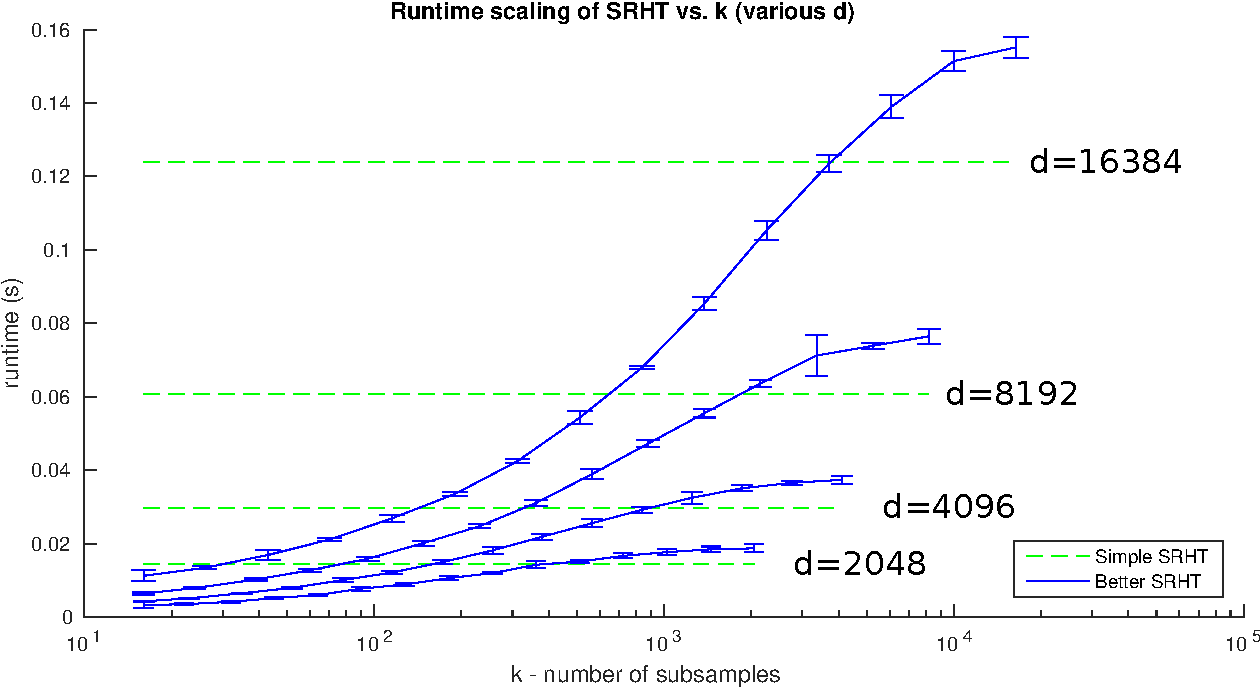
\includegraphics[width=0.8\textwidth]{figures/srht_matlab_ref_k_scaling_trim.pdf}
   \caption{{\sc matlab} reference implementation of the na\"ive SRHT and the smarter SRHT (\ref{eq:srht_rec}).}
   \label{fig:srht_matlab_ref}
\end{figure}

\begin{figure}[ht!]
   \centering
   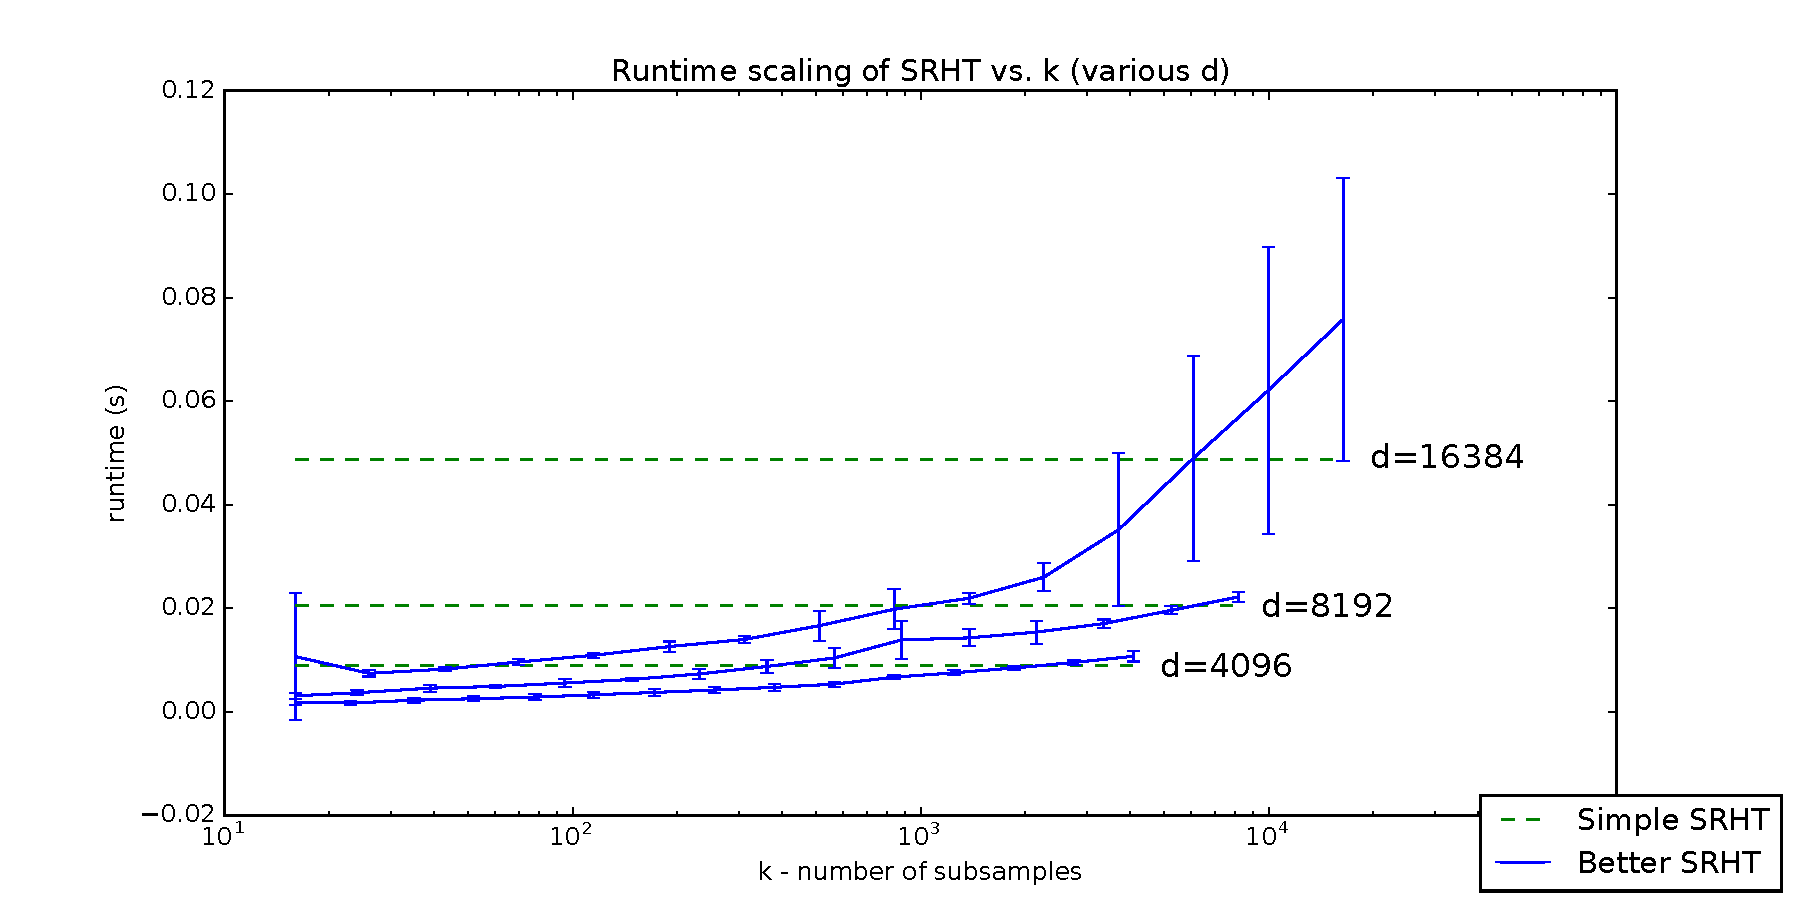
\includegraphics[width=0.9\textwidth]{figures/srht_julia_ref_k_scaling.pdf}
   \caption{Julia reference implementation of the na\"ive SRHT and the smarter SRHT (\ref{eq:srht_rec}).}
   \label{fig:srht_julia_ref}
\end{figure}

\begin{figure}[ht!]
   \centering
   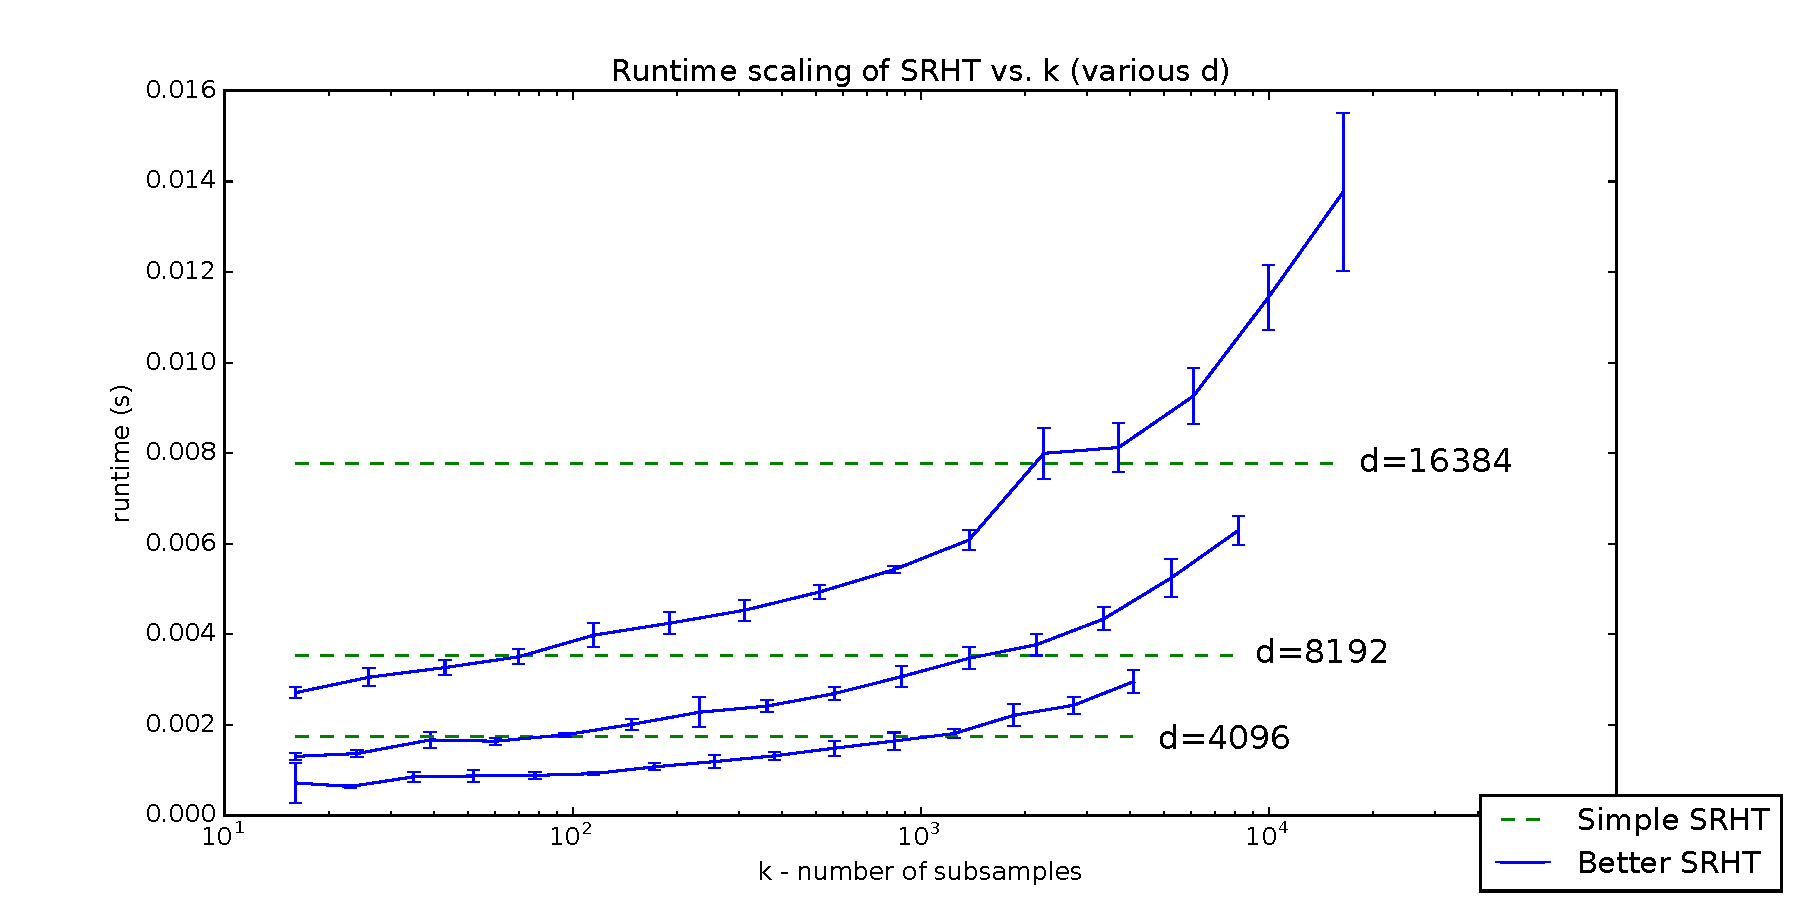
\includegraphics[width=0.9\textwidth]{figures/srht_C_k_scaling.pdf}
   \caption{Optimized $C$ implementations of the full Hadamard transform (\ref{eq:had_rec}) and smarter SRHT (\ref{eq:srht_rec}).  The optimized full Hadamard transform was used for the ``Simple SRHT''.}
   \label{fig:srht_C}
\end{figure}


\section{Discussion}
Ubaru et al. experimented with using subsampled dual BCH code matrices as sampling matrices for the RSVD \cite{ubaru2015low}.  In addition to having nice theoretical properties, dual BCH code matrices admit a fast multiplication operation via the SRHT and enjoy performance on par with Gaussian and SRFT sampling operators.

We also implemented Ailon and Liberty's SRHT algorithm \cite{ailon2009fast}, which has complexity $\mathcal{O}(d\log k)$.  To our knowledge, this is the first publicly available implementation of the SRHT that has this complexity, instead of the simple SRHT, which has complexity $\mathcal{O}(d\log d)$.  Time permitting over the summer, we may clean up, document, and publish our SRHT code under an open source license for others to use.

\bibliography{final_bib}
\bibliographystyle{siam}
 
\end{document} % every document must end with this.

%fast_decay_rsvd_compare_trim.pdf  srht_C_k_scaling.pdf      srht_matlab_ref_k_scaling_trim.pdf
%kohonen_rsvd_compare_trim.pdf   srht_julia_ref_k_scaling.pdf

